\subsection{Esempi Linguaggi Liberi}
Essendo un linguaggio libero chiuso rispetto alla concatenazione, dati:\\
$L_1 = \{a^nb^nc^j \ / \ n, j \geq 0\} $ Libero\\
$L_2 = \{a^nb^nc^n \ / \ n,j \geq 0\}$ Libero perch\'e concatenazione di $\{a^nb^n\ / \ n \geq 0 \}$ e $\{ c^j \ / \ j \geq 0 \}$, entrambi liberi\\
$L_3 = \{a^nb^nc^n \ / \ n \geq 0\}$ Non \'e libero:

Suppongo $L_3$ libero, sia $p \in \mathbb{N}^+$, $z = a^pb^pc^p$
Allora $z \in  L_3,\ |z|=3p>p$\\
Spacco z in $A=a...a,\ B = b...b, C=c...c$\\
Siano $z = uvwxy\ \land\ |vwx| \leq p \ \land\ |vx| > 0 $:
\begin{itemize}
    \item vwx \'e composto da sole a in A\\
    \item vwx \'e composto da a in A e b in B\\
    \item vwx \'e composto da sole b in B\\
    \item vwx \'e composto da b in B e c in C\\
    \item vwx \'e composto da sole c in C\\
\end{itemize} 
Considero la parola $z' = uv^0wx^0y$ 
\begin{itemize}
    \item[1.] $z' = a^kb^pc^p,\ k<p,\ z' \not\in L_3 $\\
    \item[3.] $z' = a^pb^kc^p,\ k<p,\ z' \not\in L_3 $\\
    \item[5.] $z' = a^pb^pc^k,\ k<p,\ z' \not\in L_3 $\\
    \item[2.] $z' = a^kb^jc^p,\ k<p\ \lor\ j < p ,\ z' \not\in L_3 $\\
    \item[4.] $z' = a^pb^kc^j,\ k<p\ \lor\ j < p ,\ z' \not\in L_3 $\\
\end{itemize}
Quindi visto che la parola non appartiene mai ad $L_3$ il linguaggio non \'e libero.
$\Box$\\[5pt]

\begin{tcolorbox}\begin{center}
    Quindi la classe di linguaggi liberi \textbf{non \'e chiusa rispetto all'intersezione}
\end{center}\end{tcolorbox}

$L_4 = \{a^nb^mc^{n+m} \ / \ n,m>0\}$ Libero\\
$S \rightarrow aSc | aBc$\\
$B \rightarrow bBc|bc$\\

$L_5 = \{ a^nb^mc^nd^m | n,m > 0\}$ Non libero \\
$L_6= \{ wcw^R \ / \ w \in \{a,b\}^+\}$ Libero \\
$S \rightarrow aSa | bSb | aca|bcb$

%%%%%%%%%%%%%%%%%%%%%%%%%%%%%%%%%%%%%%%%%%%%%%%%%%%%%%%%%%%%%%%%%%%%%%%%%%%%%%%%%%%%%%%%%%%%%%%
\chapter{Automi a stati finiti}

Un NFA accetta/riconosce un certo linguaggio.

Sia N un NFA, allora il linguaggio riconosciuto/accettato da N \'e il set delle parole per le quali esiste almeno un cammino dallo stato iniziale di N ad uno stato finale di N.

notare che $\forall\ a \in A,\ a\epsilon = \epsilon a = a$.

%%%%%%%%%%%%%%%%%%%%%%%%%%%%%%%%%%%%%%%%%%%%%%%%%%%%%%%%%%%%%%%%%%%%%%%%%%%%%%%%%%%%%%%%%%%%%%%
\section{Thompson construction}
\begin{center}
    \begin{tabular}{ll}
        input & regular expression r\\
        output & NFA N $\ / \ L(N) = L(r)$\\ 
    \end{tabular}
\end{center}
Gli NFA usati nei passi della costruzione hanno:
\begin{itemize}
    \item un solo stato finale\\ 
    \item non hanno archi entranti sul nodo iniziale\\ 
    \item non hanno archi uscenti dal nodo finale\\
\end{itemize}

\textbf{Lemma}: Lo NFA ottenuto dalle costruzini di Thompson ha al massimo 2k stati e 4k archi, con k lunghezza della re. r.
\textbf{Osservazione}: Ogni passo della costruzione introduce al massimo 2 nodi e 4 archi.

\begin{center}
	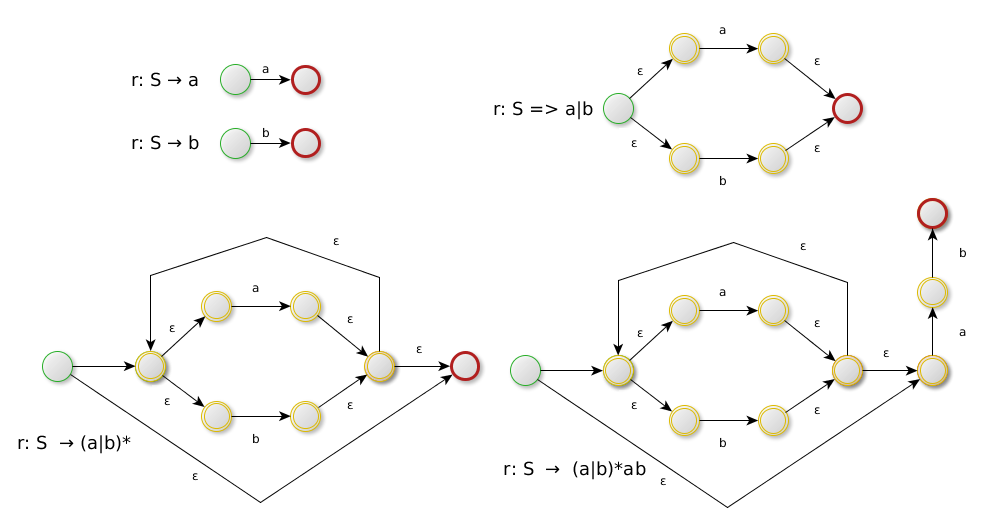
\includegraphics[scale=0.4]{Chapters/Img/c02_01.png}\\
\end{center} 
Algoritmo a complessit\'a $O(|r|)$ 

%%%%%%%%%%%%%%%%%%%%%%%%%%%%%%%%%%%%%%%%%%%%%%%%%%%%%%%%%%%%%%%%%%%%%%%%%%%%%%%%%%%%%%%%%%%%%%%
\section{Simulare un NFA}
Il backtracking consiste nel seguire un percorso e se non va bene tornare in dietro e provarne un altro finch\'e alla fine 
li provo tutti mal che vada.

$N=(S,A,move_n,S_0,F)$, S insieme stati, A degli archi, $S_0$ stato iniziale, F set stati finali, $move_n$ funzione di transizione\\
$t \in S, T \subset S$\\
$\epsilon - closure(\{ t \})$ il set degli stati S raggiungibili tramite \underline{zero o pi\'u} 
$\epsilon -transizioni$ da t (in pratica il nodo stesso e tutti i nodi raggiungibili con una $\epsilon-transition$).

Nota che $\forall t \in S,\ t\in \epsilon-closure(t)$\\
$\epsilon-closure(T) = \cup _{t \in T} \epsilon-closure(t)$

Questo algoritmo \'e pi\'u performante del backtracking.

%%%%%%%%%%%%%%%%%%%%%%%%%%%%%%%%%%%%%%%%%%%%%%%%%%%%%%%%%%%%%%%%%%%%%%%%%%%%%%%%%%%%%%%%%%%%%%%
\subsection{Algoritmo per la computazione}
Strutture dati:
\begin{itemize}
    \item pila\\
    \item bool[] alreadyOn, dimensione $|S|$\\
    \item array[][] $move_n$\\ 
\end{itemize}
\begin{lstlisting}
    for(int i = 0; i < |S|; i++){
        alreadyOn[i] = false;
    }
    closure(t, stack){
        push t onto stack;
        alreadyOn[t] = true; //posso sempre arrivare a me stesso con una epsilon-transition 
        foreach(i in move_n(t, epsilon)){
            if(!alreadyOn[i]){
                closure(i, stack);
            }
        }
    }
\end{lstlisting}

\begin{center}
	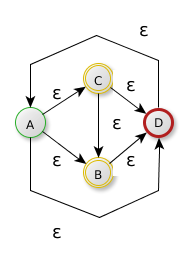
\includegraphics[scale=0.5]{Chapters/Img/c02_02.png}\\
\end{center} 

\begin{lstlisting}
    alredyOn[F F F F];
    closure(A, pila vuota)
        [A] [T F F F]
            //B non e' ancora nella pila
            closure(B, [A])
                [A, B] [T T F T]
                closure(D, [A, B])
                    [A, B, D] [T T F T]
            closure(C, [A, B, D])
                [A, B, C, D] [T T T T]
\end{lstlisting}

%%%%%%%%%%%%%%%%%%%%%%%%%%%%%%%%%%%%%%%%%%%%%%%%%%%%%%%%%%%%%%%%%%%%%%%%%%%%%%%%%%%%%%%%%%%%%%%
\subsection{Algoritmo per la simulazione di un NFA}
\begin{center}
    \begin{tabular}{ll}
        input & NFA N, w$\$$\\
        output & yes se $w \in L(N)$, no altrimenti\\ 
    \end{tabular}
\end{center}
\begin{lstlisting}
    N = (S, A, move_n, S_0, F)
    states = epsilon-closure({S_0})
    symbol = nextchar()
    while(symbol != $){
        states = epsilon-closure(Unione_{t in states} di move_n(t, symbol));
        symbol = newxtchar();
    }
    if(states intersecato F != emptyset){
        return yes;
    }
    return no;
\end{lstlisting}

%TODO GRAFO PAGINA 17

Algoritmo a complessit\'a $O(|w|(n+m))$ 


%%%%%%%%%%%%%%%%%%%%%%%%%%%%%%%%%%%%%%%%%%%%%%%%%%%%%%%%%%%%%%%%%%%%%%%%%%%%%%%%%%%%%%%%%%%%%%%
\section{DFA}
Automa a stati finiti, deterministico; una sottoclasse degli NFA che rispettano:
\begin{center}
    DFA$\overset{\Delta}{=}(S,A,move_d,s_0,F)$  \\
    $move_d \overset{\Delta}{=} (S \otimes A) \rightarrow S$\\
\end{center}
\begin{itemize}
    \item non hanno $\epsilon-transizioni$\\
    \item $\forall a \in A, s \in S,\ move_n(s,a)$ \'e un unico stato se \textbf{funzione di transizione totale} 
    (al pi\'u uno stato se \textbf{funzione di transizione parziale})\\
\end{itemize}
\begin{tcolorbox}\begin{center}
    Sink è il nodo pozzo dove confluiscono tutte le transizioni non segnate;
    viene aggiunto per rendere la funzione di transizione una funzione di transizione totale
\end{center}\end{tcolorbox}

%%%%%%%%%%%%%%%%%%%%%%%%%%%%%%%%%%%%%%%%%%%%%%%%%%%%%%%%%%%%%%%%%%%%%%%%%%%%%%%%%%%%%%%%%%%%%%
\subsection{Linguaggio riconosciuto dal DFA}
Dato il DFA D, L(D) \'e il linguaggio riconosciuto da D. \\
$L(D) = \{ w=a_1,...,a_k \ / \ \exists \text{ cammino in D dallo stato iniziale al finale}\}$.
$\epsilon \in L(D) \iff s_0 \in F$.

%%%%%%%%%%%%%%%%%%%%%%%%%%%%%%%%%%%%%%%%%%%%%%%%%%%%%%%%%%%%%%%%%%%%%%%%%%%%%%%%%%%%%%%%%%
\subsection{Simulazione di un DFA con $move_d$ totale}
\begin{center}
    \begin{tabular}{ll}
        input & w$\$$, DFA $D=(S,A,move_d,F)$\\
        output & yes se $w \in L(D)$, no altrimenti\\
    \end{tabular}
\end{center}

\begin{lstlisting}
    state = s_0;
    while(symbol != $ && state != bottom){
        //move_d(s, a) = bottom <=> move_d non e' definita su (s,a)
        state = move_d(state, symbol);
        symbol = newxtchar();
    }
    if(state \in F)
        return yes;
    return true;
\end{lstlisting}

Simulazione NFA costa $O(|w|(n+m))$
Simulazione DFA costa $O(|w|)$

%%%%%%%%%%%%%%%%%%%%%%%%%%%%%%%%%%%%%%%%%%%%%%%%%%%%%%%%%%%%%%%%%%%%%%%%%%%%%%%%%%%%%%%%%%
\section{Subset Construction}
\begin{center}
    \begin{tabular}{ll}
        input & $NFA(S^n,A,move_n, S_0 ^n,F^n)$\\ 
        output & $DFA(S^d,A,move_d, S_0 ^d,F^d)$\\
    \end{tabular}
\end{center}

\begin{lstlisting}
	S_0^d = epsilon-closure({S_0^n});	
    //raggruppo stati della epsilon closure in un unico stato S_0^d del DFA
	states = {S_0^d};
	tag S_0^d come non marcato;

	while(exist T in states non marcato){
		marco T;
		foreach(a in A){ //guardo ogni arco
			T_1 = epsilon-closure(U_{t in T} di move_n(t,a));
            //tutti gli stati raggiungibili con una a-transition da uno stato in T 
            //poi la loro epsilon closure
			if(T_1 != emptySet){
				move_d(T, a) = T_1;
		 		if(T_1 !in states){
					aggiungi T_1 a states come non marcato;
				}
			}
		}
	}

	foreach(T in states){
		if( (T intersecato F^n) != 0){
			metti T_1 in F^d;
		}
	}
\end{lstlisting}
Lo stato iniziale del DFA sar\'a la $\epsilon - closure$ dallo stato iniziale del NFA (quindi un set di stati).
Considero lo stato iniziale del NFA e lo marco in grassetto poi espando $T_0$ con la $\epsilon - closure$ dello stato iniziale. 

Dallo stato $T_0$ guardo per ogni arco gli stati in cui arrivo e li marco in grassetto ($T_1$, $T_2$, ...); 
poi espando quelli in grassetto guardando le rispettive $\epsilon - closure$.

Alla fine guardo i set degli stati se due set coincidono mergio gli stati.

%%%%%%%%%%%%%%%%%%%%%%%%%%%%%%%%%%%%%%%%%%%%%%%%%%%%%%%%%%%%%%%%%%%%%%%%%%%%%%%%%%%%%%%%%%
\subsection{Esercizio}
\begin{center}
	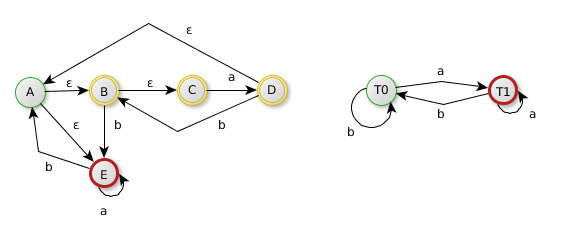
\includegraphics[scale=0.5]{Chapters/Img/c02_05.png}\\
\end{center} 

\begin{tabular}{lll}
    \textbf{States}                                 &   \textbf{a}        &     \textbf{b} \\
    T0 = $\{$ \textbf{A} B C E $\}$                 &   T1                &     T2  = T0\\
    T1 = $\{$ A B C \textbf{D E} $\}$               &   T1                &     T0 \\
    T2 = $\{$ \textbf{A} B C \textbf{E} $\}$ = T0 (quindi T0 va in T0 tramite b) & come T0 & come T0 \\
\end{tabular}

%%%%%%%%%%%%%%%%%%%%%%%%%%%%%%%%%%%%%%%%%%%%%%%%%%%%%%%%%%%%%%%%%%%%%%%%%%%%%%%%%%%%%%%%%%
\subsection{Esercizio}
\begin{center}
	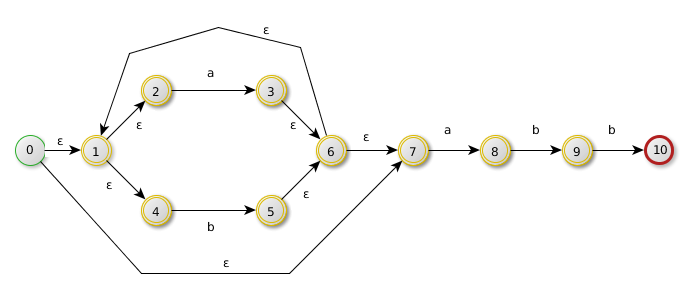
\includegraphics[scale=0.5]{Chapters/Img/c02_03.png}\\
\end{center} 

\begin{tabular}{lll}
    \textbf{States}                                 &   \textbf{a}        &     \textbf{b} \\
    $S_0^d = \{$ \textbf{0} 1 2 4 7 $\}$            &   T1                &     T2 \\
    T1 = $\{$ 1 2 \textbf{3} 4 6 7 \textbf{8} $\}$  &   T1                &     T3 \\
    T2 = $\{$ 1 2 4 \textbf{5} 6 7 $\}$             &   T1                &     T2 \\
    T3 = $\{$ 1 2 4 \textbf{5} 6 7 9 $\}$           &   T1                &     T4 \\
    T4 = $\{$ 1 2 4 \textbf{5} 6 7 \textbf{10} $\}$ &   T1                &     T2 \\
\end{tabular}

\begin{center}
	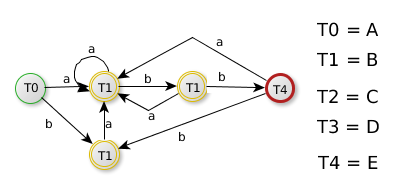
\includegraphics[scale=0.5]{Chapters/Img/c02_04.png}\\
\end{center} 

%%%%%%%%%%%%%%%%%%%%%%%%%%%%%%%%%%%%%%%%%%%%%%%%%%%%%%%%%%%%%%%%%%%%%%%%%%%%%%%%%%%%%%%%%%
\section{Partition Refinement}
\begin{tcolorbox}\begin{center}
    Guado gli archi, se tutta partizione punta ad un nodo dell'altra transizione con lo stesso non terminale allora va bene; 
    altrimenti spacco la partizione.
\end{center}\end{tcolorbox}

%%%%%%%%%%%%%%%%%%%%%%%%%%%%%%%%%%%%%%%%%%%%%%%%%%%%%%%%%%%%%%%%%%%%%%%%%%%%%%%%%%%%%%%%%%
\subsection{Algoritmo di Partition Refinement}
\begin{center}
    \begin{tabular}{ll}
        Input   &   DFA D = $\{ A,A,move_d, s_0, F\}$\\
        Output  &   partizione di S in blocchi equidistanti\\ 
    \end{tabular}
\end{center}

\begin{lstlisting}
    B_1 = F;
    B_2 = S \ F;
    P = {B_1, B_2};
    while(exists B_i, B_j in P, exists a in A, B_i e'' partizionabile rispetto a (B_j, a)){
        sostituire B_i in P con split(B_i, (B_j, a));
    }
\end{lstlisting}

%%%%%%%%%%%%%%%%%%%%%%%%%%%%%%%%%%%%%%%%%%%%%%%%%%%%%%%%%%%%%%%%%%%%%%%%%%%%%%%%%%%%%%%%%%
\subsection{Esempio}

\begin{center}
	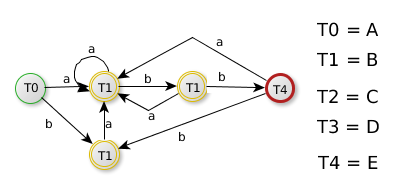
\includegraphics[scale=0.5]{Chapters/Img/c02_04.png}\\
\end{center} 

\begin{tabular}{ll}
    $\{$ A B C D $\}$ $\{$ E $\}$                       & Considero le partizioni dei terminali e non terminali \\  
    $\{$ A B C D $\}$ $\{$ E $\}$                       & Con a-transizione non esco dal primo set\\  
    $\{$ A B C $\}$ $\{$ D $\}$ $\{$ E $\}$             & Con b-transizione vado da D in E (e A B C non vanno in E con b-transizioni)\\  
    $\{$ A B C $\}$ $\{$ D $\}$ $\{$ E $\}$             & Con a-transizione non esco\\    
    $\{$ A C $\}$ $\{$ B $\}$ $\{$ D $\}$ $\{$ E $\}$   & Con b-transizione vado da B in D e gli altri no quindi splitto \\
    $\{$ A C $\}$ $\{$ B $\}$ $\{$ D $\}$ $\{$ E $\}$   & vanno bene \\
\end{tabular}\\[5pt]

Rinomino  $\{$ A C $\}$ $\{$ B $\}$ $\{$ D $\}$ $\{$ E $\}$ in $t_1,\ t_2,\ t_3,\ t_4 $

\begin{center}
	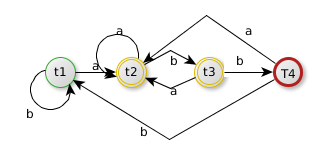
\includegraphics[scale=0.5]{Chapters/Img/c02_06.png}\\
\end{center} 

%%%%%%%%%%%%%%%%%%%%%%%%%%%%%%%%%%%%%%%%%%%%%%%%%%%%%%%%%%%%%%%%%%%%%%%%%%%%%%%%%%%%%%%%%%
\section{Algoritmo di minimizzazione di DFA}
\begin{center}
    \begin{tabular}{ll}
        Input   &   DFA \textbf{D} = $\{ S,A,move_d, s_0, F\}$ con $move_d$ totale\\
        Output  &   minimo DFA (\textbf{min(D)}) che riconosce lo stesso linguaggio del primo\\ 
    \end{tabular}
\end{center}

\begin{lstlisting}
    P = PartitionRefinement(DFA D);
    // P = (B_1, ..., B_k);
    foreach(B_i in P){
        var t_i;            //do un nome alla partizione
        if(s_o in B_i){
            t_i e'' iniziale per min(D);    //setto lo stato iniziale di min(D)
        }
    }

    foreach(B_i in P, B_i in F){
        t_i e'' lo stato finale di min(D);  //setto lo stato finale di min(D)
    }

    foreach( (B_i, a, B_j) tale che esiste s_i in B_i tali che move_d(s_i, a) = s_j){
        //per ogni tupla (stato, arco, stato) faccio la rispettiva transizione in min(D)
        setto una transizione temporanea in min(D) da t_i a t_j secondo il simbolo a;
    }

    foreach(dead state t_i){
        rimuovere t_i e tutte le transizioni da/verso t_i;
    }
    tutti i temporanei residui (sia stati che transizioni) sono gli stati e le transizioni di min(D);
\end{lstlisting}
Complessit\'a $O(nlgn)$.

%%%%%%%%%%%%%%%%%%%%%%%%%%%%%%%%%%%%%%%%%%%%%%%%%%%%%%%%%%%%%%%%%%%%%%%%%%%5
\subsection{Esempio}

\begin{center}
	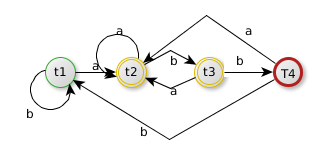
\includegraphics[scale=0.5]{Chapters/Img/c02_06.png}\\
\end{center} 
Arrivato qua: rinominati $\{$ A C $\}$ $\{$ B $\}$ $\{$ D $\}$ $\{$ E $\}$ in $t_1,\ t_2,\ t_3,\ t_4 $,
applico la minimizzazione del DFA.

\begin{center}
	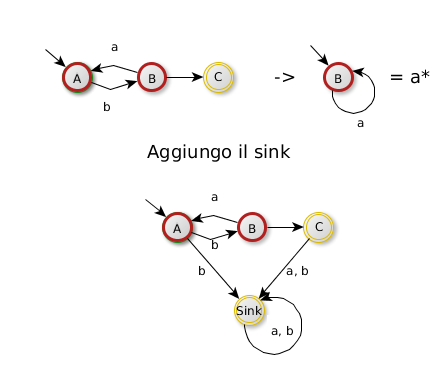
\includegraphics[scale=0.5]{Chapters/Img/c02_07.png}\\
\end{center} 

Ho le partizioni $\{A,\ B\}$, $\{C,\ sink\}$, applico partition refinement ma sono gi\'a partizionati correttamente.

\begin{center}
	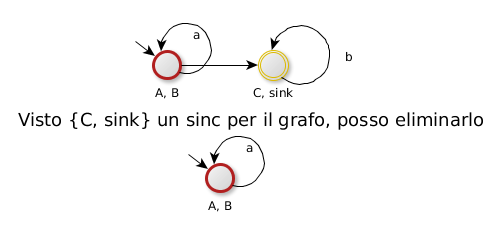
\includegraphics[scale=0.5]{Chapters/Img/c02_08.png}\\
\end{center} 

%%%%%%%%%%%%%%%%%%%%%%%%%%%%%%%%%%%%%%%%%%%%%%%%%%%%%%%%%%%%%%%%%%%%%%%%%%%5
\subsection{Esempio}
Sia $r=(a|b)*a(a|b)(a|b)$, per determinare il minimo DFA di riconoscimento di L(r) posso usare Thompson e spararmi in faccia o andare
a naso.

\begin{center}
	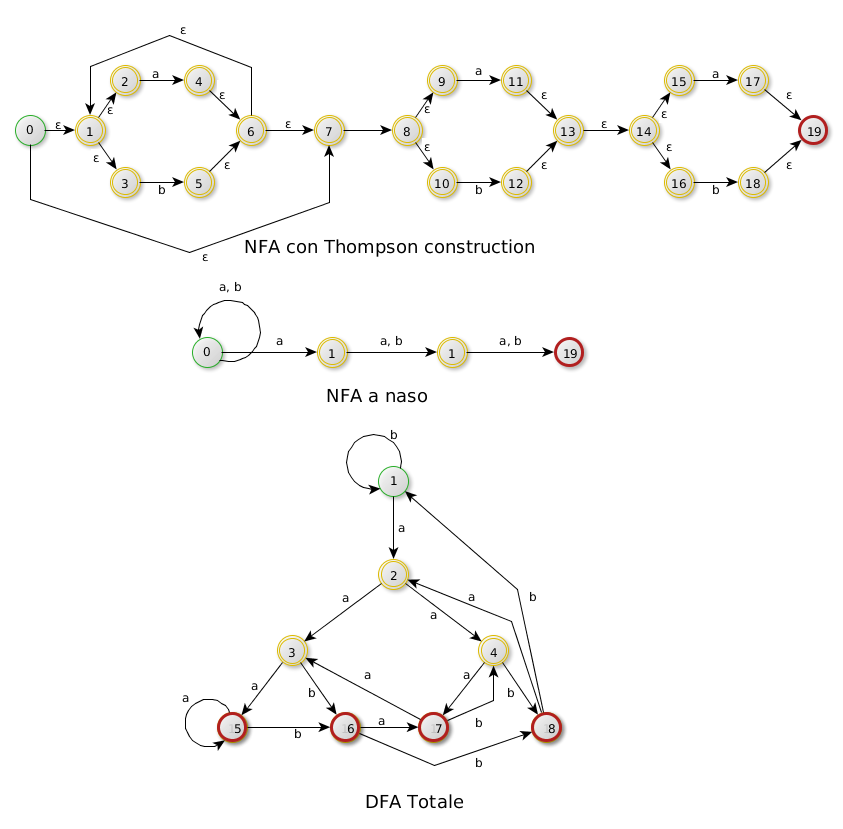
\includegraphics[scale=0.5]{Chapters/Img/c02_09.png}\\
\end{center} 

%%%%%%%%%%%%%%%%%%%%%%%%%%%%%%%%%%%%%%%%%%%%%%%%%%%%%%%%%%%%%%%%%%%%%%%%%%%%%%%%%%%%%%%%%%%%%%%%%%%%%%%%%%%%%%%%%%%5
\subsection{Lemma}
Lemma: $\forall n \in \mathbb{N}^+,\ \exists\ $ un NFA con (n+1) stati il cui minimo DFA equivalente ha almeno $2^n$ stati.\\

Dim: 
\begin{center}
	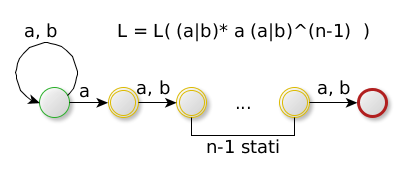
\includegraphics[scale=0.5]{Chapters/Img/c02_10.png}\\
\end{center} 

Per assurdo suppongo esista un DFA minimo con meno di $2^n$ stati.\\
Osservo che esistono $2^n$ possibili parole di lunghezza n con simboli $\{ a, b\}$.
$\implies \exists\ w_1 \not = w_2 \ / \ |w_1| = |w_2| = n $ e il loro riconoscimento conduce allo stesso stato del DFA.
$\implies$ esiste almeno una posizione per cui $w_1 \ e\ w_2$ differiscono (considero quella pi\'u a destra).\\

$w_1 = w_1'ax$, $w_2 = w_2'bx$ iniziano diversi ma finiscono con x entrambe.
Considero $w_1'' = w_1'ab^{n-1}$ $w_2'' = w_2'bb^{n-1}$ raggiungo uno stato finale t; la seconda parola per\'o non appartiene al 
linguaggio, nonostante possa comunque raggiungere lo stato t. Pertanto contraddiciamo che t sia finale.
%TODO

%%%%%%%%%%%%%%%%%%%%%%%%%%%%%%%%%%%%%%%%%%%%%%%%%%%%%%%%%%%%%%%%%%%%%%%%%%%%%%%%%%%%%%%%%%%%%%%%%%%%%%%%%%%%%%%%%%%5
\section{Ricapitolando}
\begin{center}
	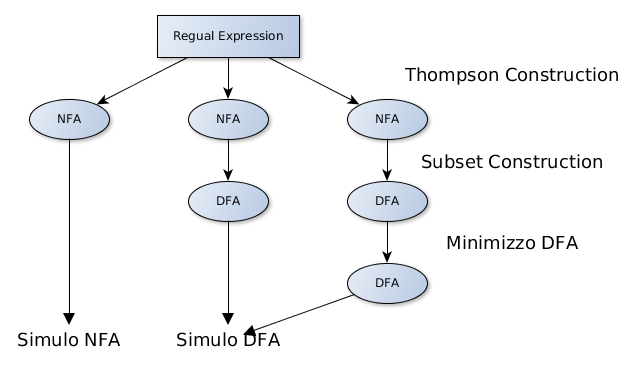
\includegraphics[scale=0.5]{Chapters/Img/c02_11.png}\\
\end{center} 

\begin{tabular}{|l|l|l|}
\hline
Algoritmo   &   Complessit\'a nello spazio  &   Complessit\'a nel tempo\\
\hline
Thompson Construction   &   $O(|r|)$    &   $O(|r|)\ ||\ O(n_n+m_n)$\\
Simulazione NFA         &   -           &   $O(|w|(n_n+m_n))$       \\
Subset Construction     &   -           &   $O(n_d |A| (n_n + m_n))$\\
Minimazzazione DFA      &   -           &   $O(n_d lg(n_d))$        \\
Simulazione DFA         &   -           &   $O(|w|)$                \\
\hline
\end{tabular}

%%%%%%%%%%%%%%%%%%%%%%%%%%%%%%%%%%%%%%%%%%%%%%%%%%%%%%%%%%%%%%%%%%%%%%%%%%%%%%%%%%%%%%%%%%%%%%%%%%%%%%%%%%%%%%%%%%%5
\section{Da DFA a Grammatica Regolare}
Dato un DFA D voglio trovare una grammatica regolare G tale che L(G) = L(D). 
Se ho una transizione $A \rightarrow B$ con una a-transizione diventer\'a $A \rightarrow aB$. Segno il nome del nodo che sto considerando
prima della freccia e, dopo la freccia, il non terminale ed il nodo destinazione. Se ho un nodo foglia C avr\'o  $C \rightarrow \epsilon$.

Se invece ho una grammatica regolare (della forma ...) e voglio trovare un DFA D $/\ L(G) = L(D)$, faccio il procedimenti inverso di prima;
se ottengo un NFA basta fare Subset Construction.

%%%%%%%%%%%%%%%%%%%%%%%%%%%%%%%%%%%%%%%%%%%%%%%%%%%%%%%%%%%%%%%%%%%%%%%%%%%%%%%%%%%%%%%%%%%%%%%%%%%%%%%%%%%%%%%%%%%5
\subsection{Esempio}
$L=\{ w \ / \ w \in \{ a, b \} ^* \&\& |a|\ pari,\ |b|\ dispari \}$, L \'e regolare?
\begin{center}
	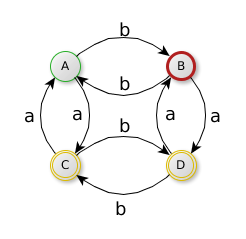
\includegraphics[scale=0.5]{Chapters/Img/c02_12.png}\\
\end{center} 
S\'i \'e regolare.

%%%%%%%%%%%%%%%%%%%%%%%%%%%%%%%%%%%%%%%%%%%%%%%%%%%%%%%%%%%%%%%%%%%%%%%%%%%%%%%%%%%%%%%%%%%%%%%%%%%%%%%%%%%%%%%%%%%5
\subsection{Esempio}
$L=\{ w \ / \ w \in \{ a, b \} ^* \&\& |a|=|b|\}$, L \'e regolare?
\begin{center}
	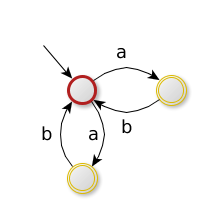
\includegraphics[scale=0.5]{Chapters/Img/c02_13.png}\\
\end{center} 
Non potr\'a mai essere regolare, per il pumping lemma per i linguaggi regolari.

%%%%%%%%%%%%%%%%%%%%%%%%%%%%%%%%%%%%%%%%%%%%%%%%%%%%%%%%%%%%%%%%%%%%%%%%%%%%%%%%%%%%%%%%%%%%%%%
\section{Pumping Lemma per Linguaggi Regolari}

Sia L un linguaggio regolara
$\implies \exists\ p \in \mathbb{N}^+ \ / \ \forall\ z \in L \ / \ |z| > p$,
$\exists\ u,v,w \ / \ $:
\begin{itemize}
    \item[i)] $z = uvw \land$\\
    \item[i)] $|uv| \leq p \land$\\
    \item[i)] $|v| > 0,\ \forall i \in \mathbb{N},\ u v^i w \in L$\\
\end{itemize}

Dim:

L \'e regolare quindi pu\'o essere riconosciuto da un automa a stati finiti.
Sia D il min DFA $\ / \ L(D) = L,\ p = |S|$, allora i cammini pi\'u lunghi che non passano pi\'u di una volta nel medesimo 
stato hanno al pi\'u lunghezza (p-1).
Allora se $z \in L$ con $|z|>p$, z \'e riconosciuta tramite un cammino che attraversa almeno due volte uno stato. 

%%%%%%%%%%%%%%%%%%%%%%%%%%%%%%%%%%%%%%%%%%%%%%%%%%%%%%%%%%%%%%%%%%%%%%%%%%%%%%%%%%%%%%%%%%%%%%%%%%%%%%%%%%%%%%%%%%%5
\subsection{Negazione testi Pumping Lemma per linguaggi regolari}
$\forall p \in \mathbb{N}^+ \ / \ \exists\ z \in L \ / \ |z| > p.\ \forall\ uvw $
$z = uvw \land |uv| \leq p \land |v| > 0) \implies \exists\ i \in \mathbb{N} \ / \ u v^i w \not\in L) $

Lemma: $L=\{a^nb^n \ / \ n \geq 0\}$ non \'e regolare\\
Dim: Assumo per assurdo che L sia regolare, dato p un qualunque numero positivo e $z= a^p b^p $ allora
$\forall\ uvw \ / \ z = uvw \land |uv| \leq p \land |v| > 0$ (la stringa v contiene solo (e almeno una) \lq a\rq ).

allora $uv^2w$ ha la forma $a^{p+k}b^p,\ k > 0$
allora $uv^2w \not\in L$ il che contraddice il Pumping Lemma per linguaggi regolari.

%%%%%%%%%%%%%%%%%%%%%%%%%%%%%%%%%%%%%%%%%%%%%%%%%%%%%%%%%%%%%%%%%%%%%%%%%%%%%%%%%%%%%%%%%%%%%%%%%%%%%%%%%%%%%%%%%%%5
\subsection{Esercizio}
$L_1 = \{ w \ / \ w \in \{ a, b \}^* \text{e contiene almeno una occorrenza di \lq\lq aa \rq\rq}\}$\\

$L_1$:
$A \rightarrow aA | bA | aB$\\
$B \rightarrow aC$\\
$C \rightarrow aC | bC | \epsilon $\\

$L_2 = \{ ww \ / \ \ \in \{ a,b \}^* \}$\\
non \'e libero per il pumping lemma (gi\'a dimostrato), quindi non \'e regolare.

$L_3 = \{ww^r \ / \ w \in \{ a,b \}^* \}$\\
Non \'e regolare ma libero.
$z = a^p b^p b^p a^p \in L_3$
visto che $uv < p$, uv \'e composta solo da a 
$u v^i w = a^pb^{2p}a^p \not\in L_3$ quindi non pu\'o essere regolare.

%%%%%%%%%%%%%%%%%%%%%%%%%%%%%%%%%%%%%%%%%%%%%%%%%%%%%%%%%%%%%%%%%%%%%%%%%%%%%%%%%%%%%%%%%%%%%%%%%%%%%%%%%%%%%%%%%%%5
\subsection{Esercizi di esame}
Sia $N_1$ lo NFA con stato iniziale A e finale E con la seguente funzione di transizione:

\begin{center}
    \begin{tabular}{|c|c|c|c|}
        \hline
            &   $\epsilon$      &   a           &   b           \\
        \hline
            A    &   $\{B, E\}$ &   $\o$        &  $\o$         \\
        \hline
            B    &   $\{ C \}$  &   $\o$        &  $\{ E \}$    \\
        \hline
            C    &   $\o$       &   $\{ D \}$   &  $\o$         \\
        \hline
            D    &   $\{ E \}$  &   $\o$        &  $\{ B \}$    \\
        \hline
            E    &   $\o$       &    $\{ E \}$  &  $\{ A \}$    \\
        \hline
    \end{tabular}
\end{center} 

\begin{itemize}
    \item[1)] $aa \in L(N_1)$?\\
    \item[2)] D \'e il DFA ottenuto da $N_1$, per subset construction, Q stato iniziale di D, $Q_{ab\_}$ lo stato di D che si 
    raggiunge da Q tramite il cammino ab. Dire a quale sottoinsieme degli stati di $N_1$ corrisponde $Q_{ab\_}$.\\    
\end{itemize}

1) S\'i facendo $A \rightarrow B \rightarrow C \rightarrow D \rightarrow E \rightarrow E $
2) Facendo la subset construction:

\begin{center}
    \begin{tabular}{|l|l|l|}
        \hline
                                &   a   &  b    \\
        \hline
            $Q0 = \{A,B,C,D\}$  &   Q1  &  Q0   \\
        \hline
            $Q1 = \{D,E\}$      &   Q2  &  Q0   \\
        \hline
           $Q2 = \{E\}$         &   Q2  &  Q0   \\
        \hline
    \end{tabular}
\end{center} 

